%%%%%%%%%%%%%%%%%%%%%%%%%%%%%%%%%%%%%%%%%%%%%%%%%%%%%%%%%%%%%%%%%%%%%%%%%%%%%%%%
%2345678901234567890123456789012345678901234567890123456789012345678901234567890
%        1         2         3         4         5         6         7         8

\documentclass[letterpaper, 10 pt, conference]{ieeeconf}  % Comment this line out
                                                          % if you need a4paper
%\documentclass[a4paper, 10pt, conference]{ieeeconf}      % Use this line for a4
                                                          % paper

\IEEEoverridecommandlockouts                              % This command is only
                                                          % needed if you want to
                                                          % use the \thanks command
\overrideIEEEmargins
% See the \addtolength command later in the file to balance the column lengths
% on the last page of the document



% The following packages can be found on http:\\www.ctan.org
%\usepackage{graphics} % for pdf, bitmapped graphics files
\usepackage{graphicx} % for pdf, bitmapped graphics files
%\usepackage{epsfig} % for postscript graphics files
%\usepackage{mathptmx} % assumes new font selection scheme installed
%\usepackage{times} % assumes new font selection scheme installed
%\usepackage{amsmath} % assumes amsmath package installed
%\usepackage{amssymb}  % assumes amsmath package installed
\usepackage{placeins}




\title{\LARGE \bf
Control Design to Reduce the Effects of Torsional Resonance in Coupled Systems
}

%\author{ \parbox{3 in}{\centering Huibert Kwakernaak*
%         \thanks{*Use the $\backslash$thanks command to put information here}\\
%         Faculty of Electrical Engineering, Mathematics and Computer Science\\
%         University of Twente\\
%         7500 AE Enschede, The Netherlands\\
%         {\tt\small h.kwakernaak@autsubmit.com}}
%         \hspace*{ 0.5 in}
%         \parbox{3 in}{ \centering Pradeep Misra**
%         \thanks{**The footnote marks may be inserted manually}\\
%        Department of Electrical Engineering \\
%         Wright State University\\
%         Dayton, OH 45435, USA\\
%         {\tt\small pmisra@cs.wright.edu}}
%}

%\author{Daniel M. Lofaro$^{1}$, Paul Oh$^{2}$ and Tom Chmielewski$^{3}$% <-this % stops a space
\author{Daniel M. Lofaro$^{1}$ and Tom Chmielewski$^{2}$% <-this % stops a space
%\thanks{*This work was not supported by any organization}% <-this % stops a space
\thanks{$^{1}$D. Lofaro is a Ph.D. Candidate of Electrical and Computer Engineering,
        Drexel University, 3141 Chestnut Street, Philadelphia, PA, United States of America
        {\tt\small dan@danlofaro.com}}%
%\thanks{$^{2}$P. Oh is with Faculty of Mechanical Engineering and Mechanics, Drexel Uniersity, 3141 Chestnut Street, Philadelphia, PA, United States of America
%        {\tt\small paul@coe.drexel.edu}}%
\thanks{$^{2}$T. Chmielewski is a Adjunct Faculty of Electrical and Computer Engineering,
        Drexel University, 3141 Chestnut Street, Philadelphia, PA, United States of America
        {\tt\small tchmiele@cbis.ece.drexel.edu}}%
}

\begin{document}



\maketitle
\thispagestyle{empty}
\pagestyle{empty}


\begin{abstract}
%\boldmath
Connecting two rotary mechanical devices utilizes a flexible coupler to accommodate various shaft misalignments. These couplers, including belts and gear boxes, exhibit a spring constant and a viscous damping term. The spring constant causes the system to have a resonant frequency while the damping controls its amplitude. In the frequency domain this characteristic is called Torsional Resonance (TR). The TR frequencies can not be allowed into the pass band of closed loop servo because it will cause instability.
Some conventional solutions to obtain stable operation include: reduction of the servo�s bandwidth below the TR frequencies; using stiffer, more expensive, components to increase the TR frequencies thus increasing the useable bandwidth; and using notch filters to reduce the resonant peak.
The objective of this work is provide a control solution to allow systems using elastic parts, including loose belt drives and plastic gears, achieve sufficient bandwidth to obtain their desired performance. A model of a commercial application exhibiting the TR characteristic has been made using Matlab and Simulink.
A test rig has been constructed with a brushless DC motor and a system able to control the location of the TR frequencies. This test rig is controlled by a hard real time target control system which accepts control through Matlab and Simulink.
The techniques described by Bigley and Rizzo and non-linear Sliding Mode Control (SMC), which has shown to reduce the error at resonance by approximately 50dB, is desired to be modeled and implemented on the physical system. The ability to reduce the effects of TR using electrical control allows mechanical system implementation using less costly components while achieving the desired specifications.
\end{abstract}

\IEEEpeerreviewmaketitle

\section{Introduction}

When connecting two rotary mechanical devices a coupler is used. These include the use of 1:1 flexible shaft couplers, to compensate for possible shaft misalignments, as well as belts, and gear boxes. In theory it is desired to have the given coupler be perfectly rigid, every degree the actuator turns the connected load will turn to its precise location denoted by the input and the gear ratio. For a coupler to be perfectly rigid the latter must be true for all time. In reality gear boxes and couplers are not perfectly rigid and have spring and damping terms associated with them. The spring constant causes the system to have two resonant frequencies collectively called the Torsional Resonance (TR). The TR frequencies, which are referred to as the resonant frequency, $\omega_r$, and the anti-resonant frequency, $\omega_{ar}$, can not fall within the pass-band of the closed loop servo because it will cause instability.  Fig.~\ref{fig:couple} shows a diagram of a coupled system exhibiting TR. The ideal system can be reduced to a single acting inertia of $J_a+J_L$ while the system exhibiting TR is connected by a spring damper system thus that reduction can not be made.  Our goal is to demonstrate a controller that uses commonly measured states (such as motor position) to reduce the effects of TR on coupled systems.

\begin{figure}[t]
  \centering
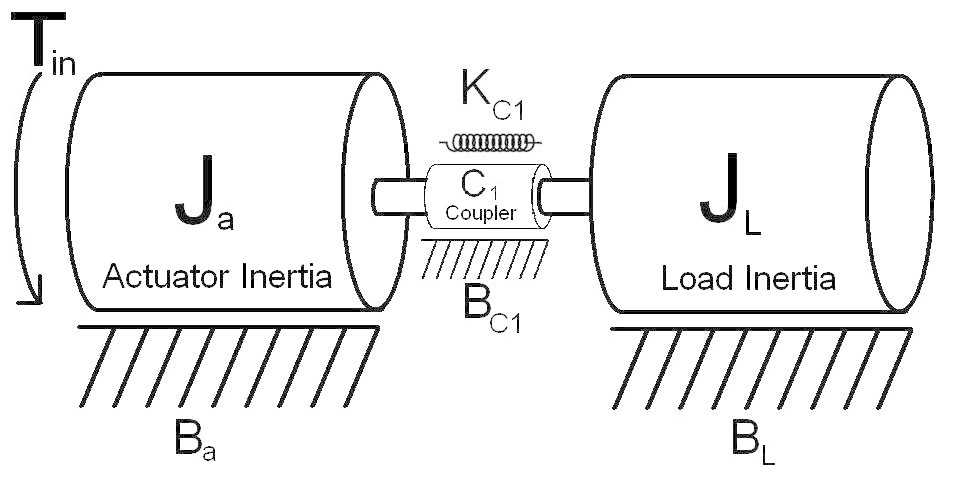
\includegraphics[width=1.0\columnwidth]{./pix/couple.png}
  \caption{System exhibiting TR. In an ideal
system (without TR) the load can be represented as a single acting inertia $(J_a+J_L)$.  The system exhibiting TR is connected by a
spring damper system thus that reduction can not be mad}
  \label{fig:couple}
\end{figure}

This paper 
Section~\ref{sec:back} gives a brief overview of TR and the contemporary ways of reducing its effects.
Section~\ref{sec:trModel} models a system exhibiting TR. 
Section~\ref{sec:load} shows the effects of TR on the system.
Section~\ref{sec:meth} goes through two methos of reducing the effects of TR (one linear and one non-linear method) where
Section~\ref{sec:re} demonstrates the method described by Rizzo and
Section~\ref{sec:smc} demonstrates a sliding-mode control based method.
Section~\ref{sec:results} show and discusses the results of both methods and 
Section~\ref{sec:con} gives final thoughts.



\section{Background}\label{sec:back}
The ideal frequency response of a coupled system, with motor position $\theta_a$ as the output and motor torque $T_{in}$ as the input, can be found in Fig.~\ref{fig:desBode} (left). 
The magnitude plot exhibits a $-40\frac{dB}{dec}$ slope with corresponding phase of $-180^o$.
The frequency response of the system exhibiting TR can be found in Fig.~\ref{fig:desBode} (right). 
It can be noted that at resonance there is a peak. This peak reduces the gain margin of the system. The phase also changes around the resonance which reduces the phase margin.  
We define "\textit{load switching}" as an offset in the $-40\frac{dB}{dec}$ slope that occurs between $\omega_{ar}$ and $\omega_r$, see Fig.~\ref{fig:trBode}.

Contemporary ways of reducing the effects of TR include:
\begin{itemize}
\item Reducing the servo's bandwidth so it does not include the TR frequencies. 
\item Increasing the couplers spring constant $K_c$ via using higher quality and anti backlash mechanical couplers and gearboxes to push the TR frequencies higher. 
\item Using notch filters to reduce the resonant peak. as well as active damping methods\cite{5730488}.   
\end{itemize}

Reducing the bandwidth of the servo means that the designed system will not be able to respond as quickly to an input stimulus. Using higher quality and anti-backlash mechanical couplers and gearboxes will give you greater bandwidth but will also include a higher materials price tag. It is also important to note that the use of notch filters is only useful in systems where the TR does not change. Most systems that have TR present tend to have nonlinear, and time varying, elements, including dynamic loads, that will cause the TR frequency to change thus making the notch filter less effective in the ideal case.  None of the latter methods address the problem of load switching.

Rizzo et. al.\cite{bigley1978resonance} (circa 1978) presented a state feedback technique for, as they describe it, ``\textit{eliminating the destabilizing effect of mechanical resonance in feedback control systems}.''  The goal of their research was to make a wide band high performance closed loop servo system. In their research Bigley and Rizzo found a relationship between the torque, or current, on the DC motor and the velocity of the shaft. They found that when the current is at its maximum the velocity is at a minimum, no matter where the resonance or anti resonance occurs, see Fig.~\ref{fig:re}. Thus feeding back the velocity and torque states would compensate for the effects of TR no matter where it occurs even when the parameters of the system changes.

Sliding mode control (SMC) is a good candidate method to reduce the effects of TR as stated by Korondi et. al.\cite{681228}. This is because SMC is a robust control method that is able to properly control a system even when parameters are not precisely known.   The main idea about SMC is that you are able to make a control that will guarantee the performance of a system in $u$ and $x$, see Fig.~\ref{fig:smcSliding}, within a given error $\psi$ and $\epsilon$ respectively. When using SMC one, or more, parameters are chosen to be unknown. The unknown parameters are given a range that they are able to be between and still have the system perform properly.

\begin{figure}[t]
  \centering
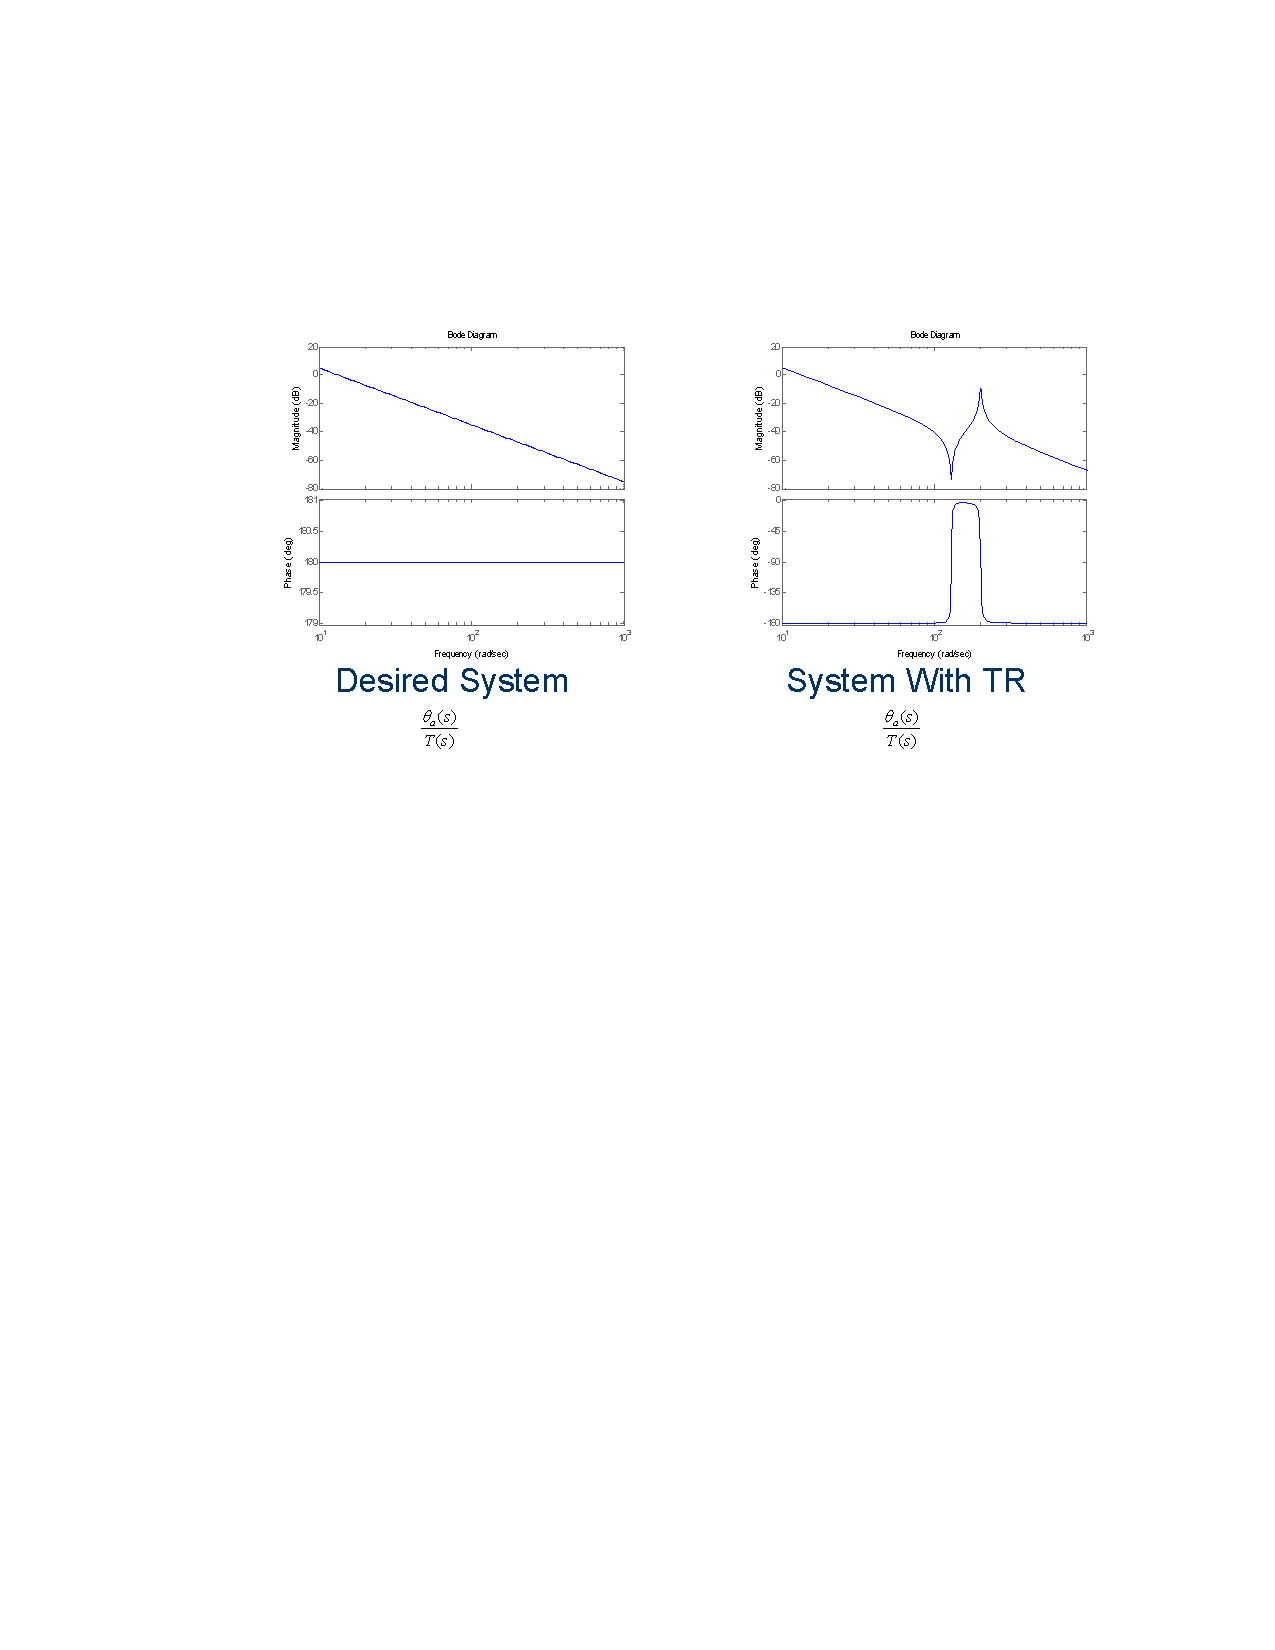
\includegraphics[width=1.0\columnwidth]{./pix/desBode.pdf}
  \caption{Frequency Response of desired coupled system (Left), Frequency response of system
exhibiting TR (Right)}
  \label{fig:desBode}
\end{figure}







\section{Torsional Resonance Model}\label{sec:trModel}
A system with TR typically consists of three main items;
An actuator, or motor, with a given inertia, $J_a$, and damping, $B_a$, associated with it.
An inertial load, $J_L$, with a given damping, $B_L$, associated with it.
A coupler between the actuator and the load with a spring constant, $K_c$, and a damping, $B_c$, associated with it.


It is assumed that the inertia of the coupler is included in the inertia of the actuator and the load. The physical diagram of the system with TR can be found in Fig.\ref{fig:couple}. In order to find the transfer function for this system, where $T_{in}$ is the torque input and the actuator angle $\theta_a$ is the output, the physical diagram is then converted into a mechanical network, see Fig.~\ref{fig:mech}, so the system's dynamics can be written as

\begin{figure}[h]
  \centering
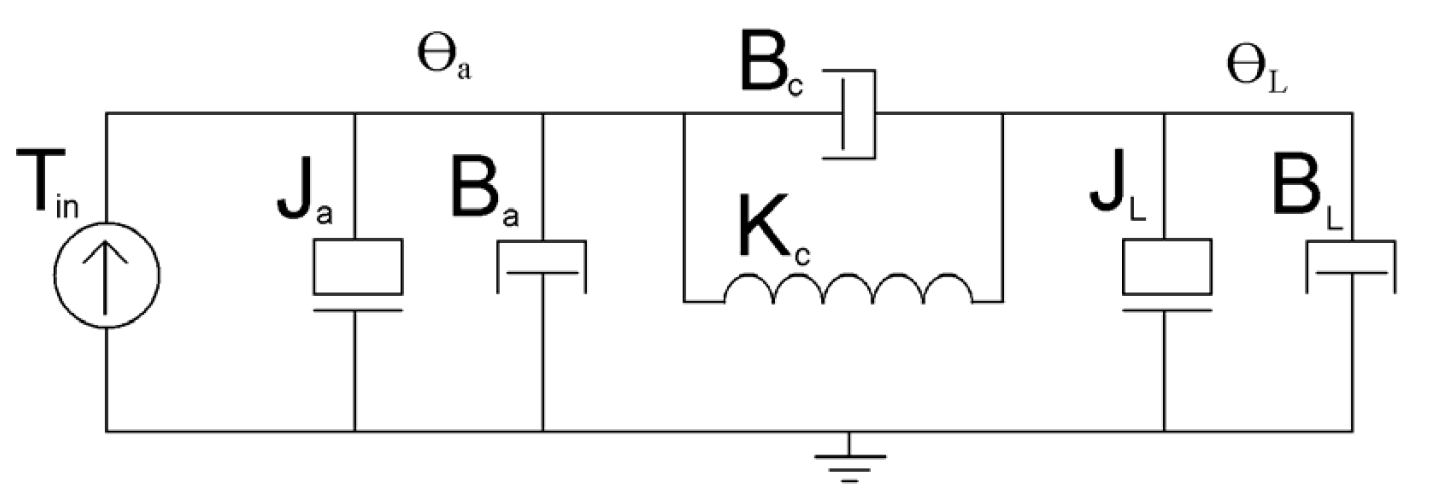
\includegraphics[width=1.0\columnwidth]{./pix/mech.png}
  \caption{Mechanical schematic drawling of system with TR}
  \label{fig:mech}
\end{figure}

\begin{equation}
%T(t) = J_a\ddot{\theta_a}+\left( B_a+B_c \right) \dot{\theta_a}=K_c\theta_a-\left(K_c\theta_L+B_c\dot{\theta_L}\right)
T(t) = J_a\ddot{\theta_a}+(B_a+B_c ) \dot{\theta_a}=K_c\theta_a-(K_c\theta_L+B_c\dot{\theta_L})
\end{equation}

The relationship between $\theta_a$ and torque, $T$, is represented as


%\begin{equation}
%T(s) = \left( (s^2J_a+sB_a+K_c+sB_c)- \frac{(K_c+sB_c)(K_c+sB_c)}{s^2J_L + sB_L + K_c +sB_c}\right) \theta_a
%\end{equation}


\begin{equation}\label{eq:tf}
\frac{\theta_a(s)}{T(s)} = \frac{  \frac{1}{J_aJ_L}\left(s^2J_L+K_c + sB_c\right)  }{s^2 \left( s^2+B_c\frac{J_a+J_L}{J_aJ_L} s + K_c \frac{J_a+J_L}{J_aJ_L} \right)}
%\frac{\theta_a(s)}{T(s)} = \frac{\frac{1}{J_aJ_L}(s^2J_L+s(B_L+B_c)+Kc)}{s^4 + K_1\frac{s^3}{J_aJ_L} + K_2\frac{s^2}{J_aJ_L} + K_3\frac{s}{J_aJ_L}}
\end{equation}

%In this system $B_a << B_L$ therefore $B_a$ is assumed to be zero.
In this system both $B_a$ and $B_L$ are assumed to be zero (Klafter et. al~\cite{chmielewski}).









The poles of a system with TR (\ref{eq:tf}) consists of a double pole at the origin and complex conjugate (CC) poles.  The CC poles are in the left half plane (LHP) as long as the following inequality is satisfied.

\begin{equation}
4K_c > B_c^2 \left( \frac{J_c+J_L}{J_aJ_L} \right)
\end{equation}


\noindent The system can represented in state space as

\begin{equation}\label{eq:ssTR}
\begin{array}{lllllll}

\left[
\begin{array}{l}
\ddot{\theta_a} 	\\ 
\dot{\theta_a}		\\
\ddot{\theta_L}	\\
\dot{\theta_L}
\end{array}
\right]



&


=

&

A

&

\left[
\begin{array}{l}
\dot{\theta_a} 	\\ 
\theta_a		\\
\dot{\theta_L}	\\
\theta_L
\end{array}
\right]

&

+

&

B

&

T(t)


\end{array}
\end{equation}


where


\begin{equation}
\begin{array}{lll}
A
&
=
&

\left[
\begin{array}{cccc}
\frac{-(B_a+B_c)}{J_a}   	& \frac{-K_c}{J_a}   	& \frac{B_c}{J_a}   		&	\frac{K_c}{J_a} \\
1 					& 0				& 0					&	0			\\
\frac{B_c}{J_L}			& \frac{K_c}{J_L}	& \frac{-(B_c+B_L)}{J_L}	& 	\frac{-K_c}{J_L} \\
0					& 0				& 0					&	1		
\end{array}

\right]


\end{array}
\end{equation}



\begin{equation}
\begin{array}{lllrrr}
B

&

=

&

\left[
\begin{array}{r}
J^{-1}_a 	\\ 
0		\\
0	\\
0
\end{array}
\right]
,
&
C
&
=
&
\left[
\begin{array}{cccc}
0 	&	1	&	0	&	0
\end{array}
\right]




\end{array}
\end{equation}


\noindent standard techniques show that the system is fully controllable and with the angular position $\theta_a$ being the only output is also fully observable.  The controllability and observability matrix are both full rank.



%A system exhibiting TR has a non-zero spring constant in the coupler $K_c$. 
The resonance and anti-resonance frequencies, $\omega_r$ and $\omega_{ar}$, are defined by the inertial load of coupled system as well as the spring constant of the coupler $K_c$.
Fig.~\ref{fig:trBode} shows the frequency response of a system that is:
\begin{itemize}
\item exhibiting TR
\item not exhibiting TR with a total inertial load of $J_a$
\item not exhibiting TR with a total inertial load of $J_a+J_L$.  
\end{itemize}
The dominant load seen by the actuator before resonance is the total inertial load ($J_a+J_L$) where after resonance it is only the actuator's inertia.  The resonance $\omega_r$ and anti-resonance $\omega_{ar}$ can be calculated by


\begin{equation}\label{eq:res}
\begin{array}{cc}

\omega_{ar} = \left(\frac{K_c}{J_L}\right)^\frac{1}{2}

&

\omega_{r} = \sqrt{\frac{K_c(J_a+J_L)}{J_aJ_L}}
\end{array}
\end{equation}

\noindent and the gain separation when going from an acting load of $J_L+J_a$ to $J_a$, as seen in Fig.~\ref{fig:trBode}, is calculated by Chmielewski \cite{chmGainSep} and is

\begin{equation}\label{eq:deltaDB}
\Delta dB = 40\mbox{log}_{10}\left(\frac{\omega_r}{\omega_{ar}}\right)
\end{equation}


\begin{figure}[ht]
  \centering
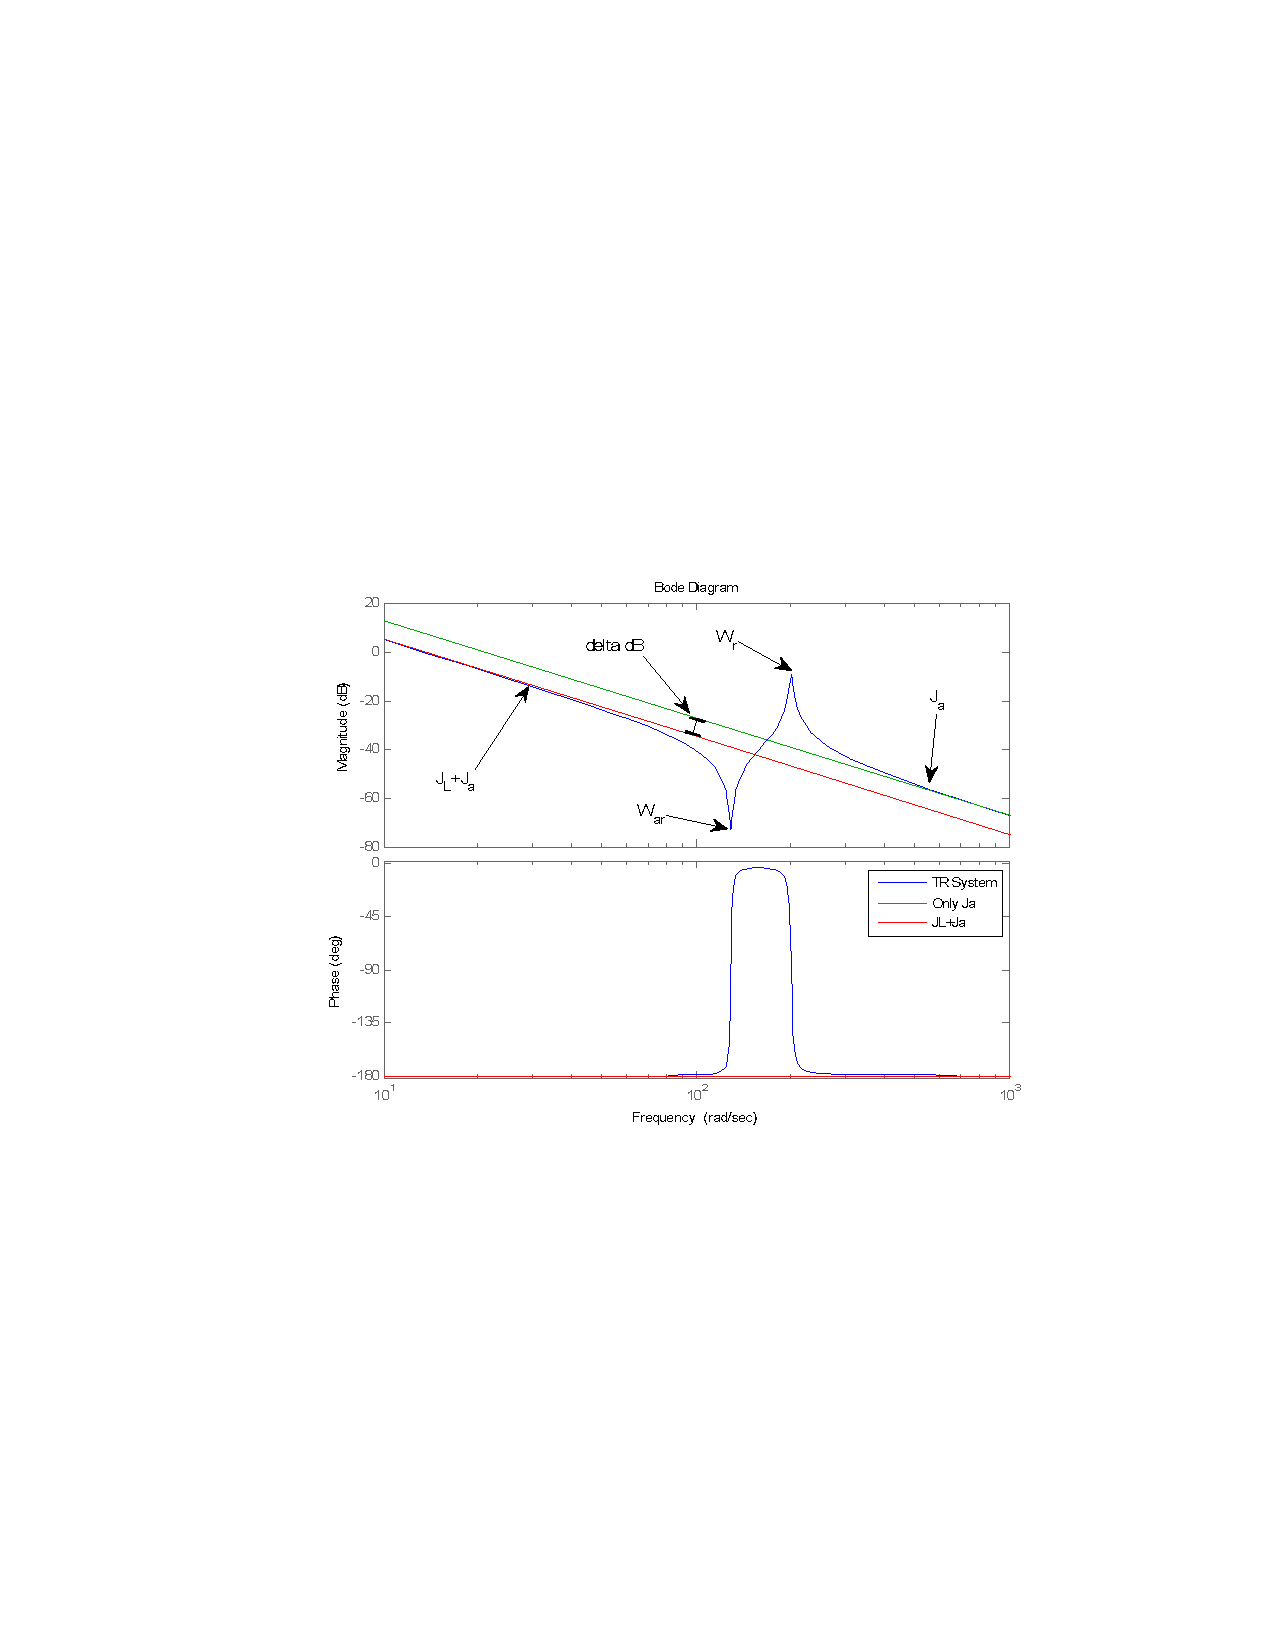
\includegraphics[width=1.0\columnwidth]{./pix/bode.pdf}
  \caption{Frequency Response Plot of System with TR (from Eq. \ref{eq:ssTR}), System with no TR with
inertial load of $J_a$, and System with no TR and inertial load of $J_a+J_L$}
  \label{fig:trBode}
\end{figure}

The anti-resonance $\omega_{ar}$ is due to the complex conjugate zeros and the resonance $\omega_r$ is due to the complex conjugate poles.  The anti-resonance will always precede the resonance.
\section{Effects of TR}\label{sec:load}
\subsection{Effect as Seen at the Actuator}
The dipping and peaking of the magnitude of the frequency response plot of a system with TR is not the
only effect that TR has on the system. Another effect is a change in the effective load seen by the system
before $\omega_{ar}$ to after $\omega_r$, see Fig.~\ref{fig:trBode}. Before the $\omega_{ar}$ the acting inertial load on the system is the sum of the
actuator�s inertial load, $J_a$, and the load�s inertial load, $J_L$. This is a second order system with a slope of
negative $40\frac{dB}{dec}$ on the frequency response plot. After the $\omega_{r}$ the acting inertial load is only the
actuator�s inertia, $J_a$, which also defines a second order system with a slope of negative $40\frac{dB}{dec}$ on the
frequency response plot. The latter characteristics can be seen in the frequency response plot in Fig.~\ref{fig:trBode}.

\noindent Transfer function $\frac{\theta_{a1}(s)}{T(s)}$ is for a mass spring damper system with effective load of $J_a+J_L$, ideal coupler (pre-$\omega_{ar}$)

\begin{equation}
\frac{\theta_{a1}(s)}{T(s)}=\frac{1}{(J_a+J_L)s^2}
\end{equation}

\noindent Transfer function $\frac{\theta_{a2}(s)}{T(s)}$ is for a mass spring damper system with effective load of $J_a$, ideal coupler (post-$\omega_{r}$)
\begin{equation}
\frac{\theta_{a2}(s)}{T(s)}=\frac{1}{J_as^2}
\end{equation}


It can be noted that there is an offset between the frequency responses of the second order estimations of
the system with TR when going from before the $\omega_{ar}$ to after the $\omega_{r}$ when looking at the magnitude in $dB$ of
the response. 
This offset is known as gain separation
Gain separation is the resulting effect of the load switching around $\omega_{ar}$ and $\omega_r$.
Fig.~\ref{fig:trBode} shows an example of gain separation in the frequency response of the system with TR.
System with TR is Eq.~\ref{eq:tf} using values from Table~\ref{table:defaultVals}.  
In addition the frequency responses of systems without TR and having the effective loads of $J_L+J_a$ and $J_a$ are also shown.
This clearly shows gain separation due to load switching.

\begin{center}
	\begin{table}
	\caption{Values used for TR model based on the PITTMAN\textsuperscript{\texttrademark} N2314 series brushless DC servo motor and a custom inertial load/coupler}
	\begin{center}
  \begin{tabular}{ c | c | c | c }

    					& Inertia 'J' 								&	Damping 'B' 												&	Spring 'K'  									\\ 
    					& ($oz-in-sec^2$)							&	($\frac{oz-in}{krpm}$)							&	$\frac{oz}{in}$) 							\\ \hline
    Actuator 	& 0.0023 											& 0																		& 0															\\ \hline
    Coupler 	& 0 													& 0.005 															& 55														\\ \hline
    Load 			& 0.0033 											& 0																		& 0															\\

  \end{tabular}
  \end{center}
  \label{table:defaultVals}
  \end{table}
\end{center}





\subsection{Effect on Velocity}

When there is a step torque command input to the system, like that seen in Fig.~\ref{fig:torqueIn} (top), the output velocity
exhibits an oscillatory behavior. The frequency of oscillation is expected to be equal to $\omega_r$ of the system
from Eq.~\ref{eq:tf}. Therefore this should have a ripple frequency of 201.4 rad/sec, 32.1 Hz.

\begin{figure}[ht]
  \centering
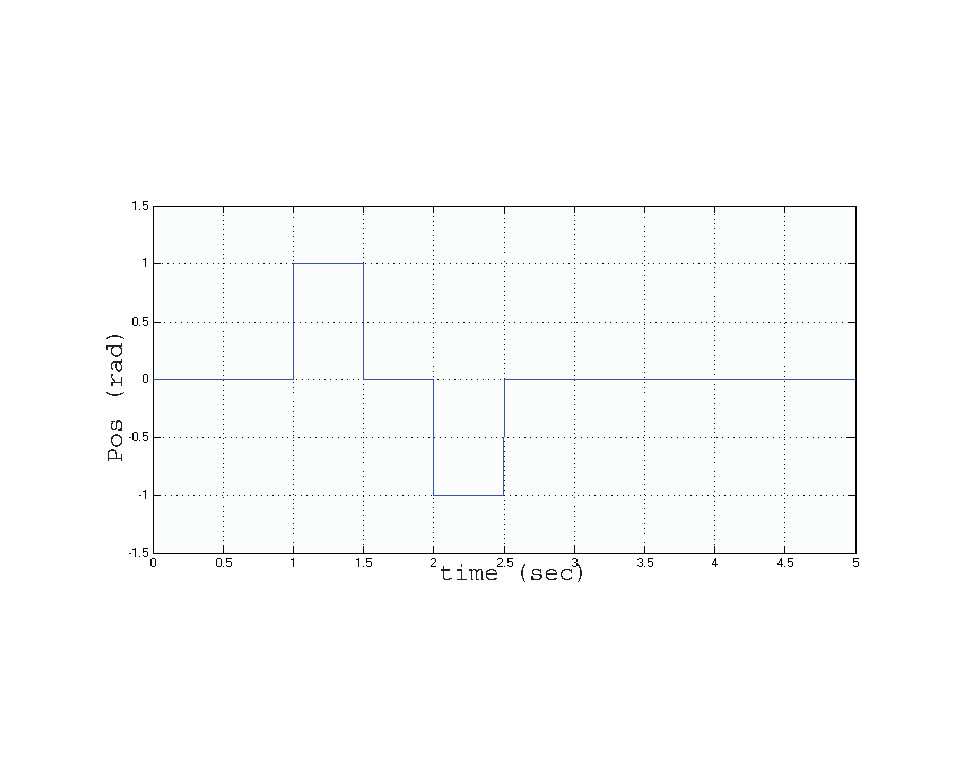
\includegraphics[width=1.0\columnwidth]{./pix/posIn2.pdf}\\
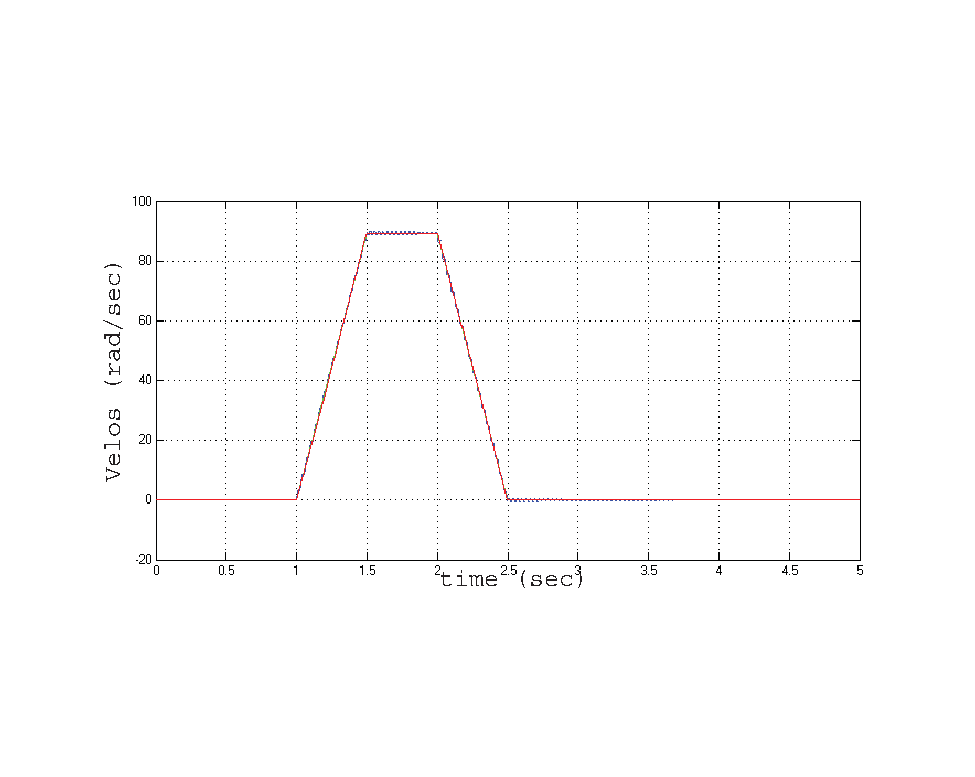
\includegraphics[width=1.0\columnwidth]{./pix/velosOut2.pdf}
  \caption{(TOP) Step Torque Input to TR System. Vertical Axis is Magnitude, Horizontal
Axis is Time in sec.  (BOTTOM) Angular Velocity of the Actuator Shaft of the system with TR (Yellow), Angular Velocity
of the Actuator Shaft of the system without TR (Pink) due to the torque input. Vertical Axis is
Magnitude, Horizontal Axis is Time in sec.}
  \label{fig:torqueIn}
\end{figure}


\begin{figure}[ht]
  \centering
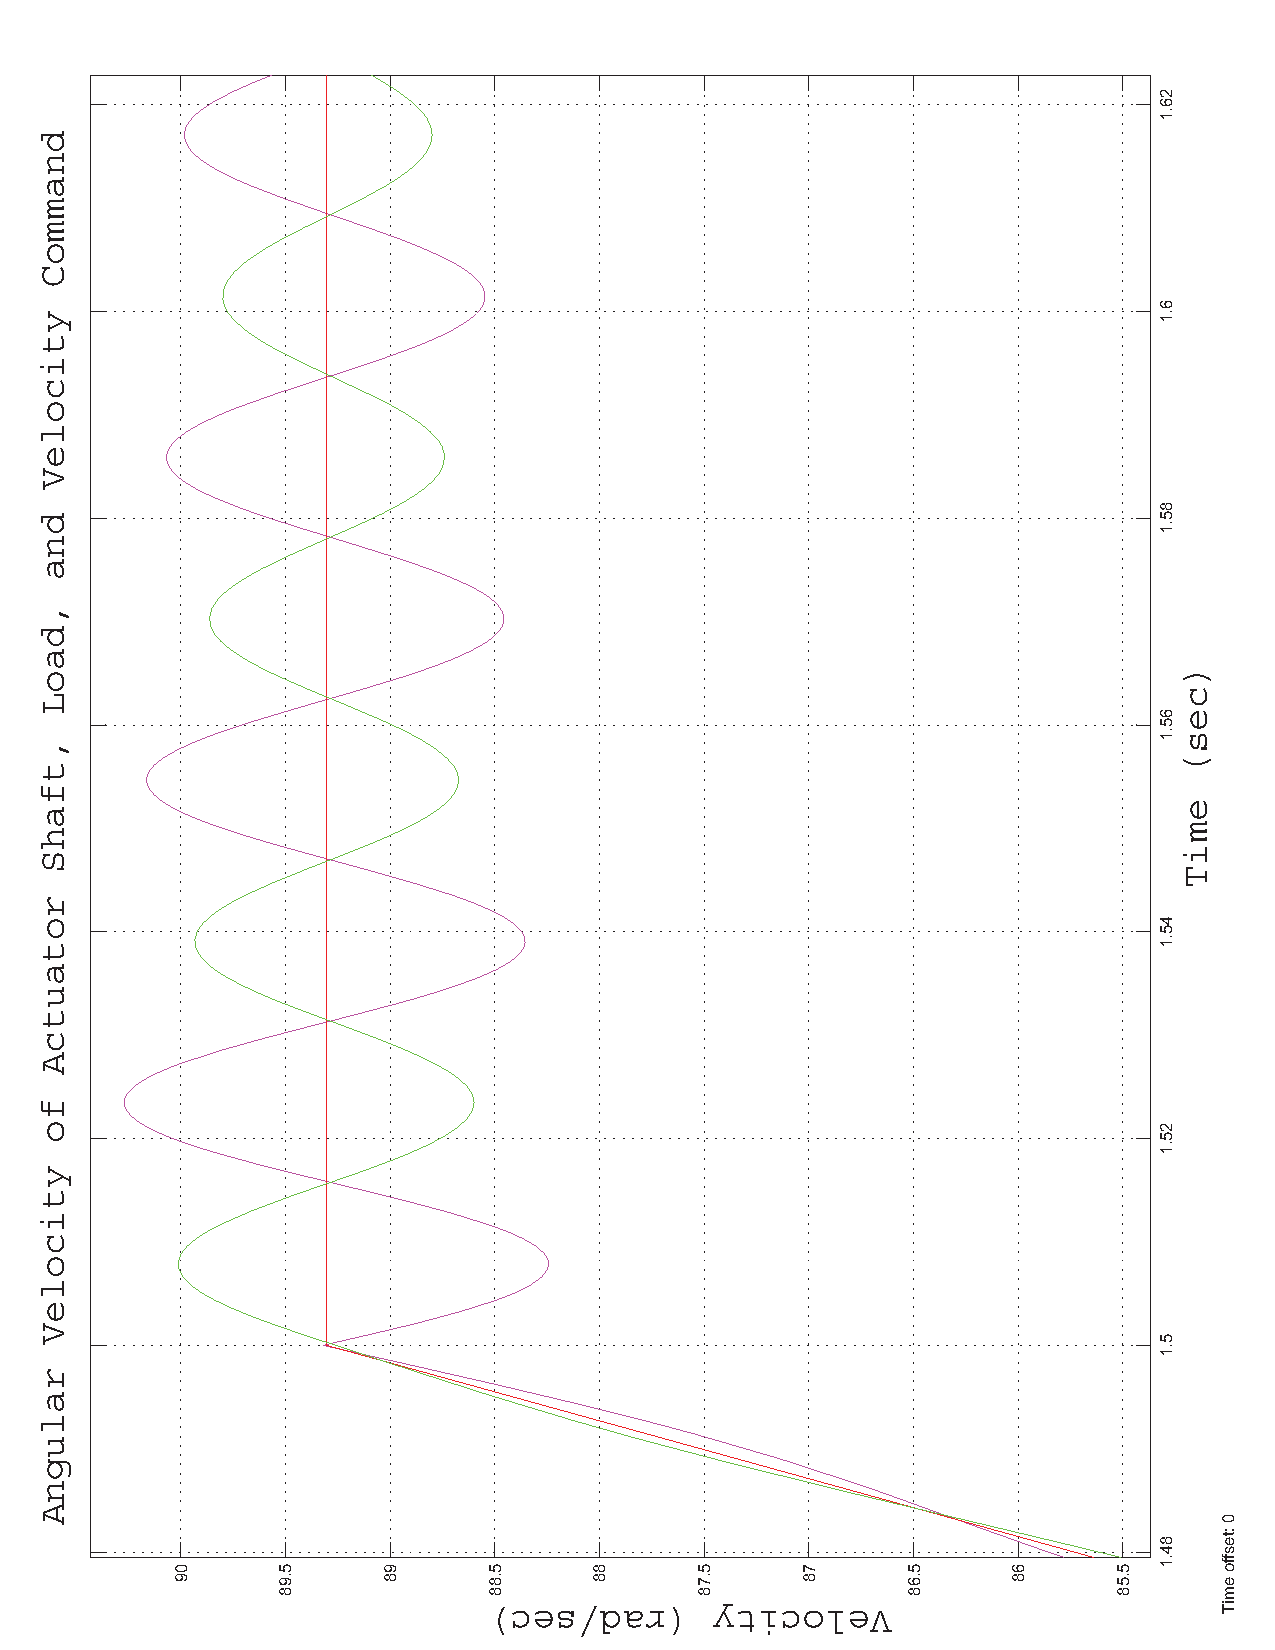
\includegraphics[angle=-90, width=1.0\columnwidth]{./pix/velosMotorAndOutputF33.pdf}
\caption{Angular velocity of the actuator shaft $\dot{\theta}_a$ for the system with TR (PURPLE), Angular velocity of the load shaft $\dot{\theta}_L$ for the system with TR (GREEN), Angular Velocity of the actuator shaft for the system without TR (RED) due to the torque input.  It is important to note that $\dot{\theta}_a$ and $\dot{\theta}_L$ are $180^o$ out of phase.}
%  \caption{Angular velocity of the actuator shaft $\dot{\theta}_a$ for the system with TR (Blue), Angular Velocity of
%the actuator shaft for the system without TR (Red) due to the torque input zoomed in from 1.5 to
%2.0 sec. Vertical Axis is Magnitude, Horizontal Axis is Time in sec}
  \label{fig:trap}
\end{figure}


Fig.\ref{fig:trap} shows Fig.~\ref{fig:torqueIn} magnified where the ideal velocity is constant (1.48 sec to 0.62 sec). The angular velocity of
the actuator shaft has a decaying sinusoid on it due to the resonance and the spring/damping.  
The period of is 0.031sec (32.2 Hz, 202.3 rad/sec). This frequency is the
same as the $\omega_r$ computed in Eq.\ref{eq:tf}, shown in Fig.~\ref{fig:trBode} and uses the values in Table~\ref{table:defaultVals}.  
This frequency is calculated by $\omega_r$ in Eq.~\ref{eq:res}.





 \section{Methodology}\label{sec:meth}
 \subsection{Resonance Equalization}\label{sec:re}
 State-variable-feedback (SVF) is a control method that uses different states of a system, such as position,
velocity, and acceleration, to create an input to achieve a desired performance. In this case the states of the
system consist of the angular position, angular velocity, and angular acceleration with the input being
torque. At this point it is pertinent to note the torque applied by a direct current (DC) motor is directly
proportional to the current through the windings of the motor. It is also pertinent to note that it is widely
known that the DC motor is a fully observable system when the output is the angular position, thus a full or
partial state observer can be made for this system. With the latter being said Rizzo et. al.\cite{bigley1978resonance}
analyzed what the effects of TR had on various parameters of the system including shaft velocity and input
current, Fig.~\ref{fig:re} is an example of some of these plots.  A key point noted is that the input current and output velocity are
almost exactly $180^o$ out of phase from one another. The importance of this is that the actuator shaft
velocity can be used as feedback in combination with the input current to compensate for the effects of the 
resonance. The latter relationship will ensure that the control is effective for changes in the resonant
frequencies.

\begin{figure}[t]
  \centering
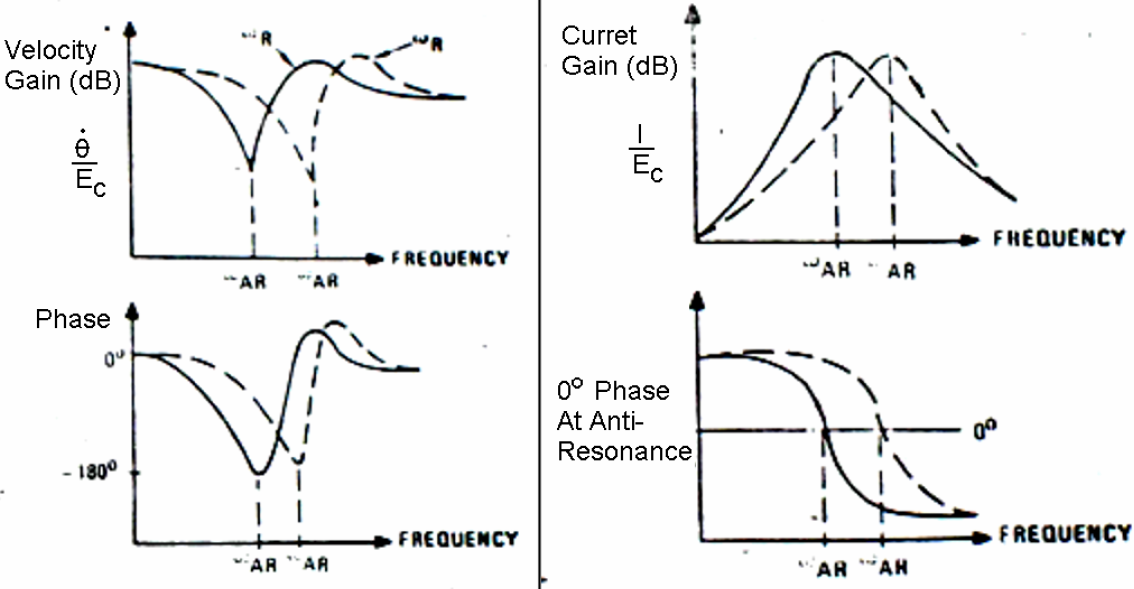
\includegraphics[width=1.0\columnwidth]{./pix/re.png}
  \caption{Plot of the Actuator Shaft Velocity and Phase (Left), Plot of the Actuator Current and
Phase (Right) around $\omega_r$ and $\omega_{ar}$\cite{bigley1978resonance}}
  \label{fig:re}
\end{figure}

Using the knowledge that the current, or torque, is about $180^o$ out of phase with the angular velocity of
the actuator Rizzo showed that ``\textit{the resonance peaking factor F is completely
eliminated}.'' Rizzo�s method is implemented in Fig.~\ref{fig:reSim} with the SVF gains of -0.2 for the current
feedback gain and 20 for the angular velocity feedback. Table~\ref{table:resultsClosedLoop} shows the maximum change 
in magnitude and phase of the frequency response plot of the
system with TR and the addition of Rizzo�s resonance equalization (RE)\cite{bigley1978resonance}.

\begin{figure}[ht]
  \centering
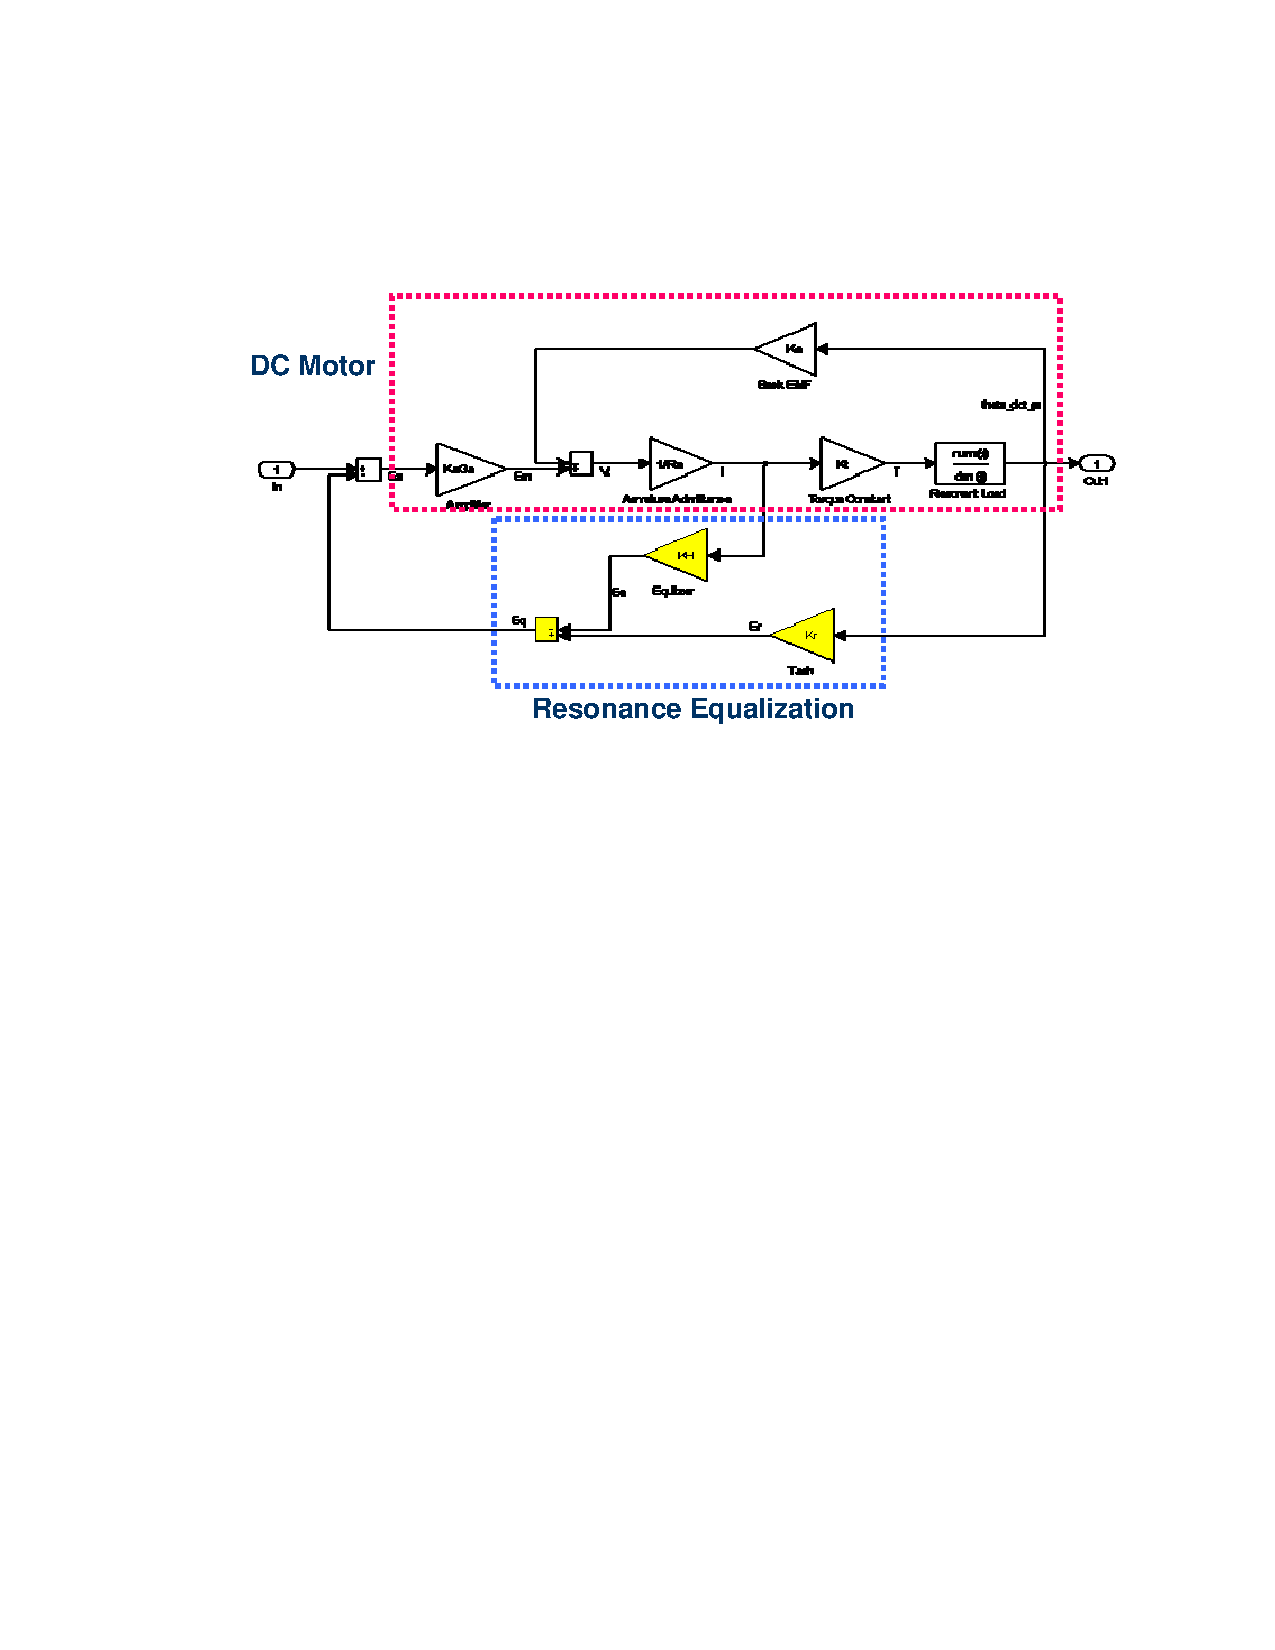
\includegraphics[width=1.0\columnwidth]{./pix/reSim.pdf}
  \caption{V.Rizzo�s resonance equalized rate loop diagram using SVF\cite{bigley1978resonance}}
  \label{fig:reSim}
\end{figure}


This results in a reduction of the resonance and anti-resonance and the corresponding phase shift.  Fig.~\ref{fig:reBode} shows the frequency response of RE on the TR system.  RE does not eliminate the load switching ($\Delta dB$) as shown in Fig.~\ref{fig:trBode}.  The motor velocity $\dot{\theta_a}$ and motor current $i_a$ states are required to implement RE.

\begin{figure}[ht]
  \centering
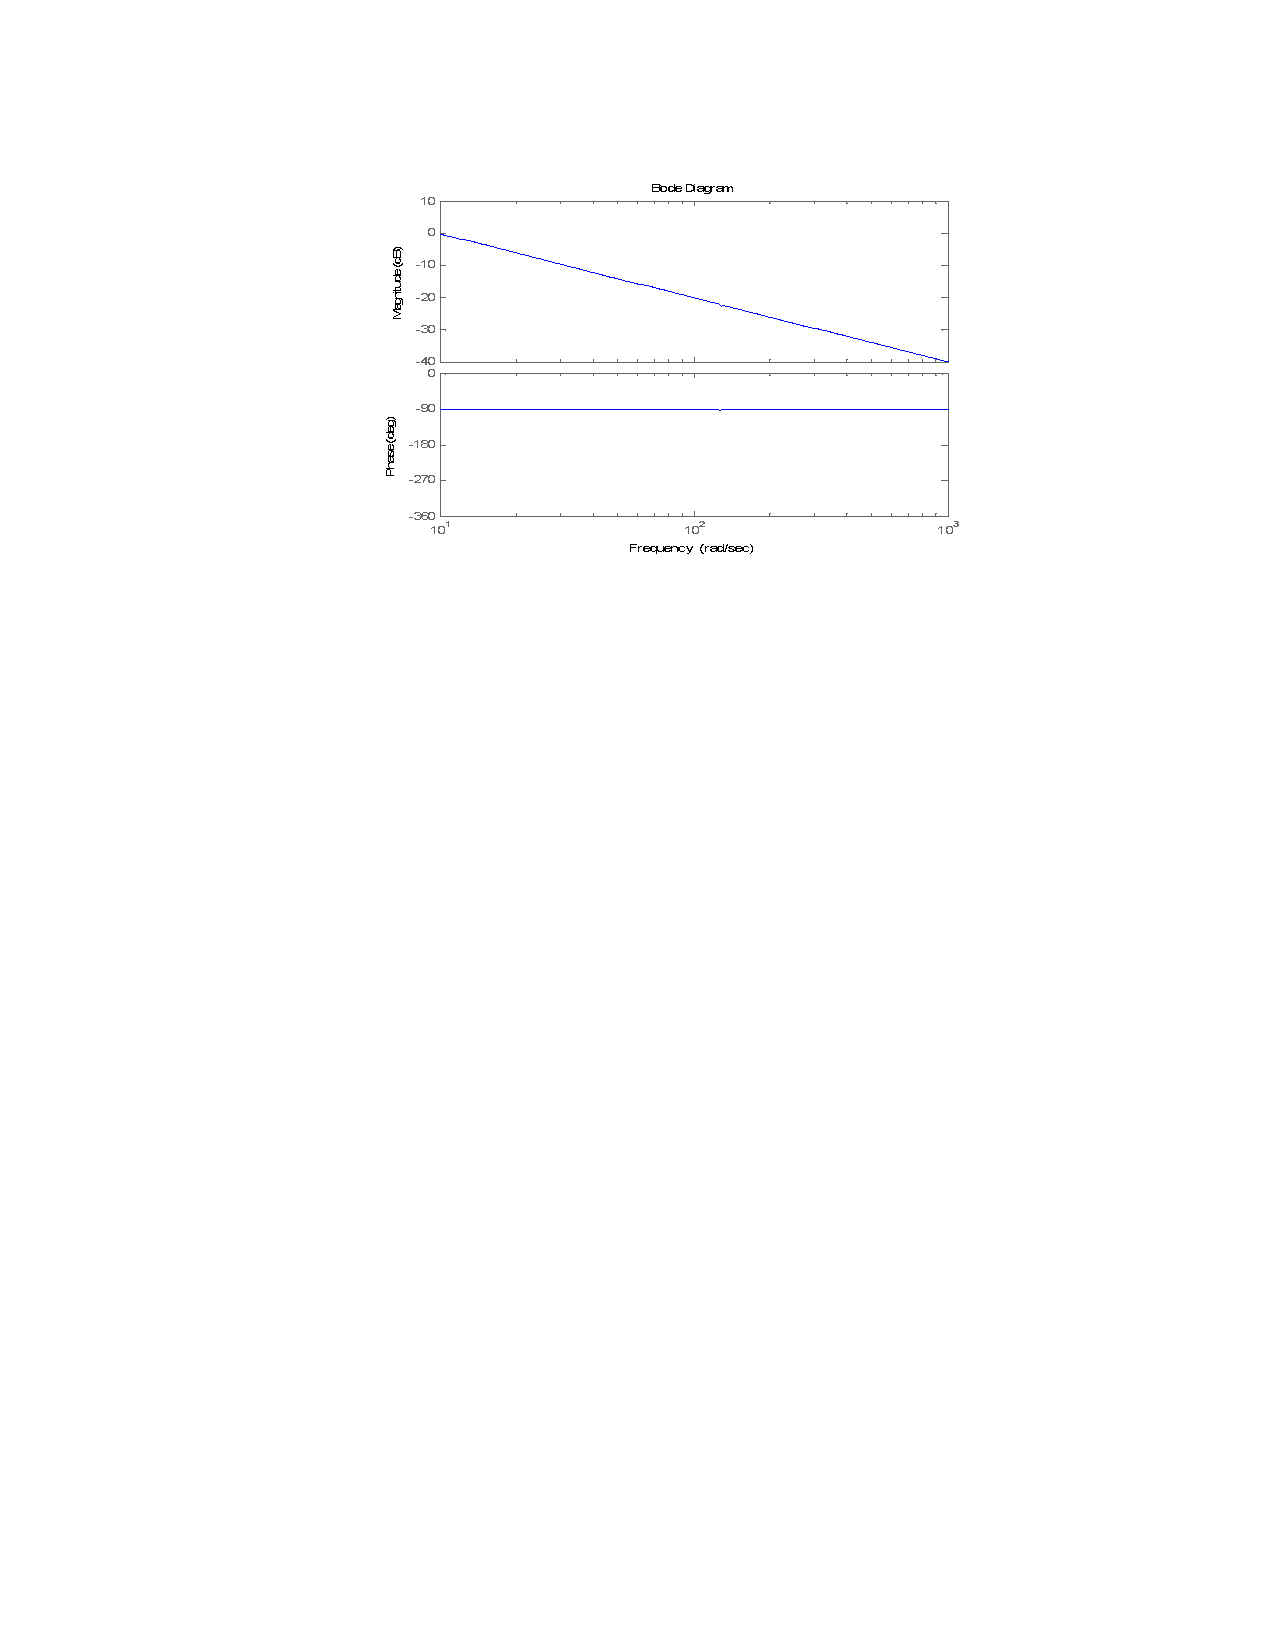
\includegraphics[width=0.8\columnwidth]{./pix/rizzoBode.pdf}
  \caption{Frequency responce of V.Rizzo�s resonance equalized TR system}
  \label{fig:reBode}
\end{figure}


\subsection{Sliding Mode Control}\label{sec:smc}
Sliding Mode Control (SMC) is a form of non-linear control that is able deal with systems that are not
linear as well as systems that have parameters which are not precisely known. The main idea about SMC is
that the performance of a system is guaranteed to be inside $u$ and $x$, see Figure 31, within a given error �
and � respectively. When using SMC one, or multiple, parameters are chosen to be unknown. These
unknown parameters are specified a range at which the given parameters are able to vary between and still
have the system perform within its given bounds $\psi$ and $\epsilon$. It is important to note that this range affects the
boundary condition $\psi$ and $\epsilon$. Once the system has entered within the boundary layer, or sliding boundary, it
will never leave it. The latter will hold true as long as the parameters which are able to vary do not go out
of the designed bounds \cite{kwatny2000nonlinear}\cite{isidori1995nonlinear}.


\begin{figure}[h]
  \centering
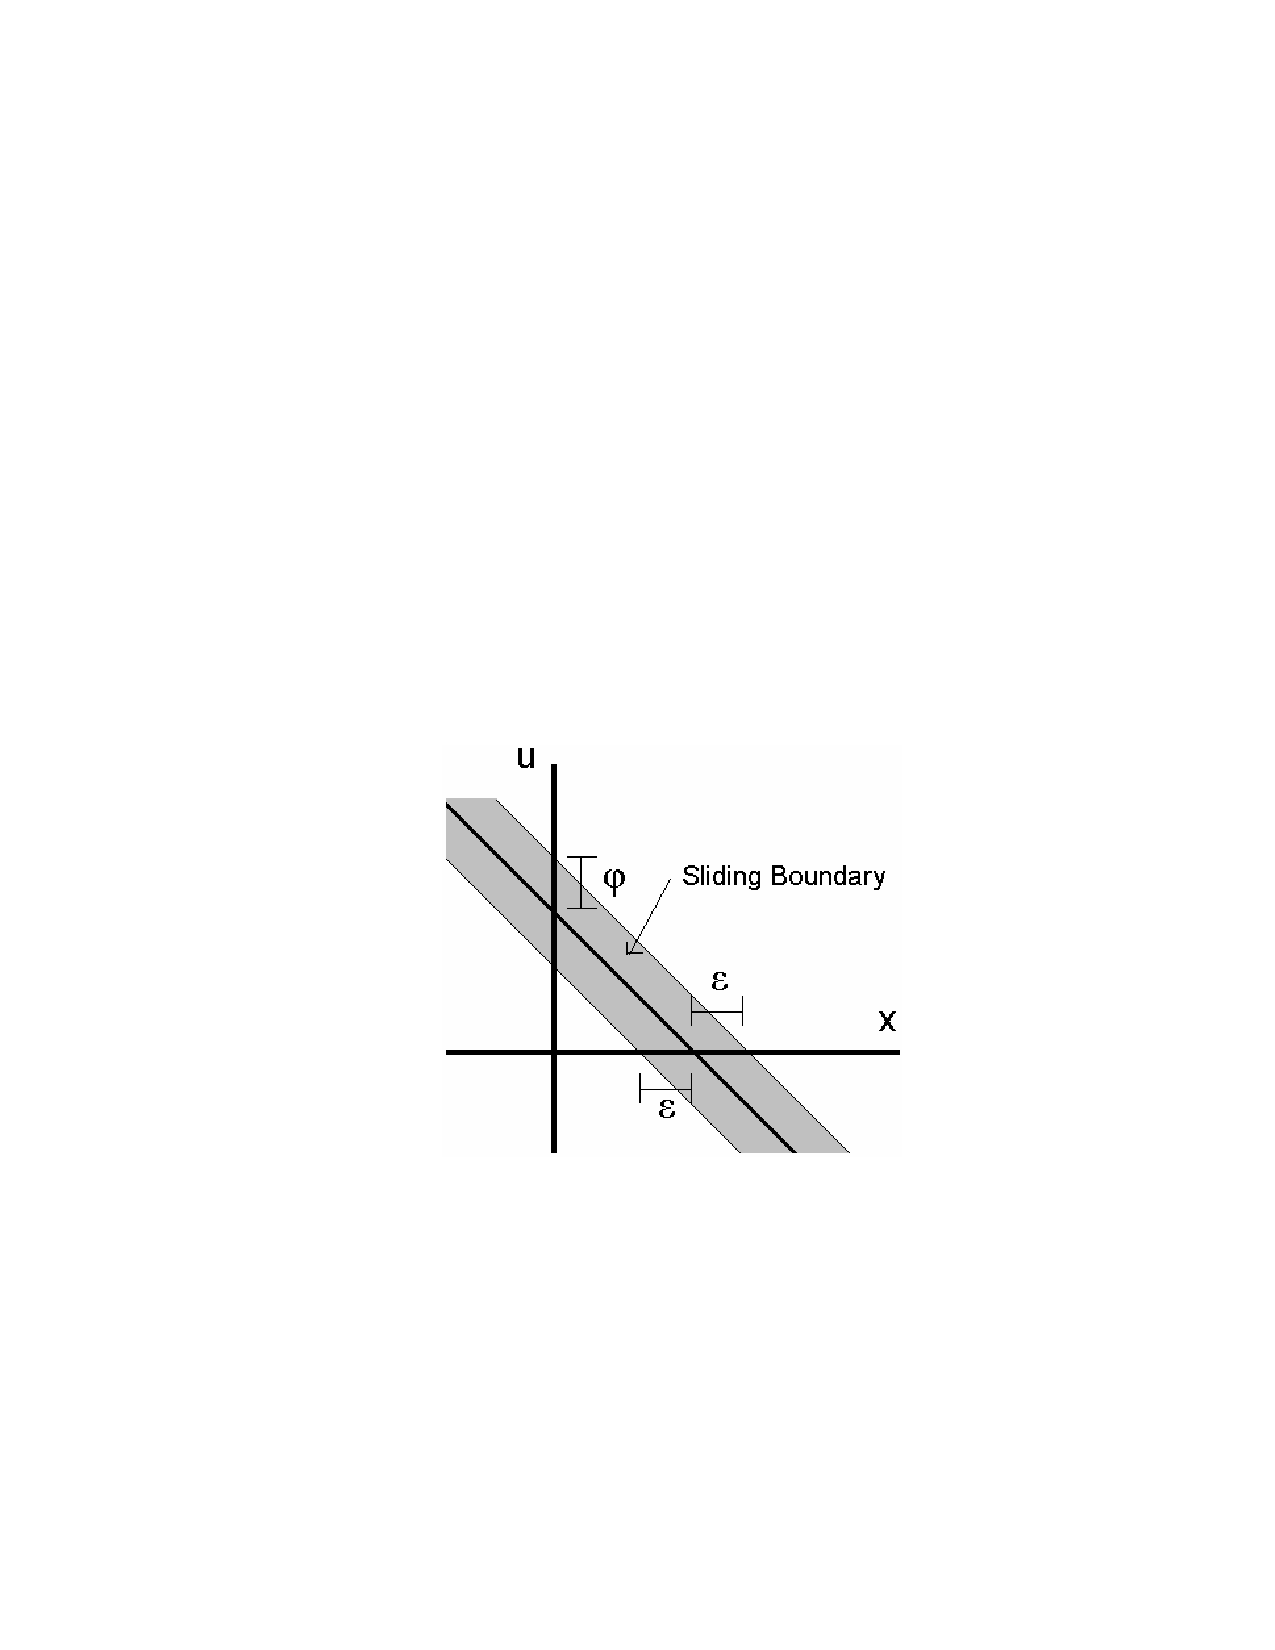
\includegraphics[width=0.7\columnwidth]{./pix/smc.pdf}
  \caption{SMC Sliding Boundary/Sliding Layer}
  \label{fig:smcSliding}
\end{figure}

The fact that a parameter can be defined to be between a given bound and still have stable control is one of
SMC�s strongest arguments for it�s use for the the reduction of TR. This is also because an exact model of
the system does not have to be made for SMC to be effective. SMC is able to take care of some of the unmodeled
dynamics including TR. Fig.~\ref{fig:trBode} shows the effective inertial load on a system with TR before $\omega_{ar}$
and after $\omega_r$. As stated previously in Fig.~\ref{fig:trBode} and Eq.~\ref{eq:deltaDB} there is an offset in the magnitude of the
frequency response due to the change in the effective load. Due to the latter the inertia has been chosen to
be the parameter to be unknown within a given bound. The inertial load will vary from $0.9J_a$ to $1.1(J_a+J_L)$
to ensure the system will always fall within the bounds of the SMC and thus stay within the sliding
boundary.

The effective load has been taken care of by letting it vary; thus the model of the TR system from Fig.~\ref{fig:couple} can be reduced and assumed to be a system with out TR, see Fig.~\ref{fig:smcSliding}.

\begin{figure}[h]
  \centering
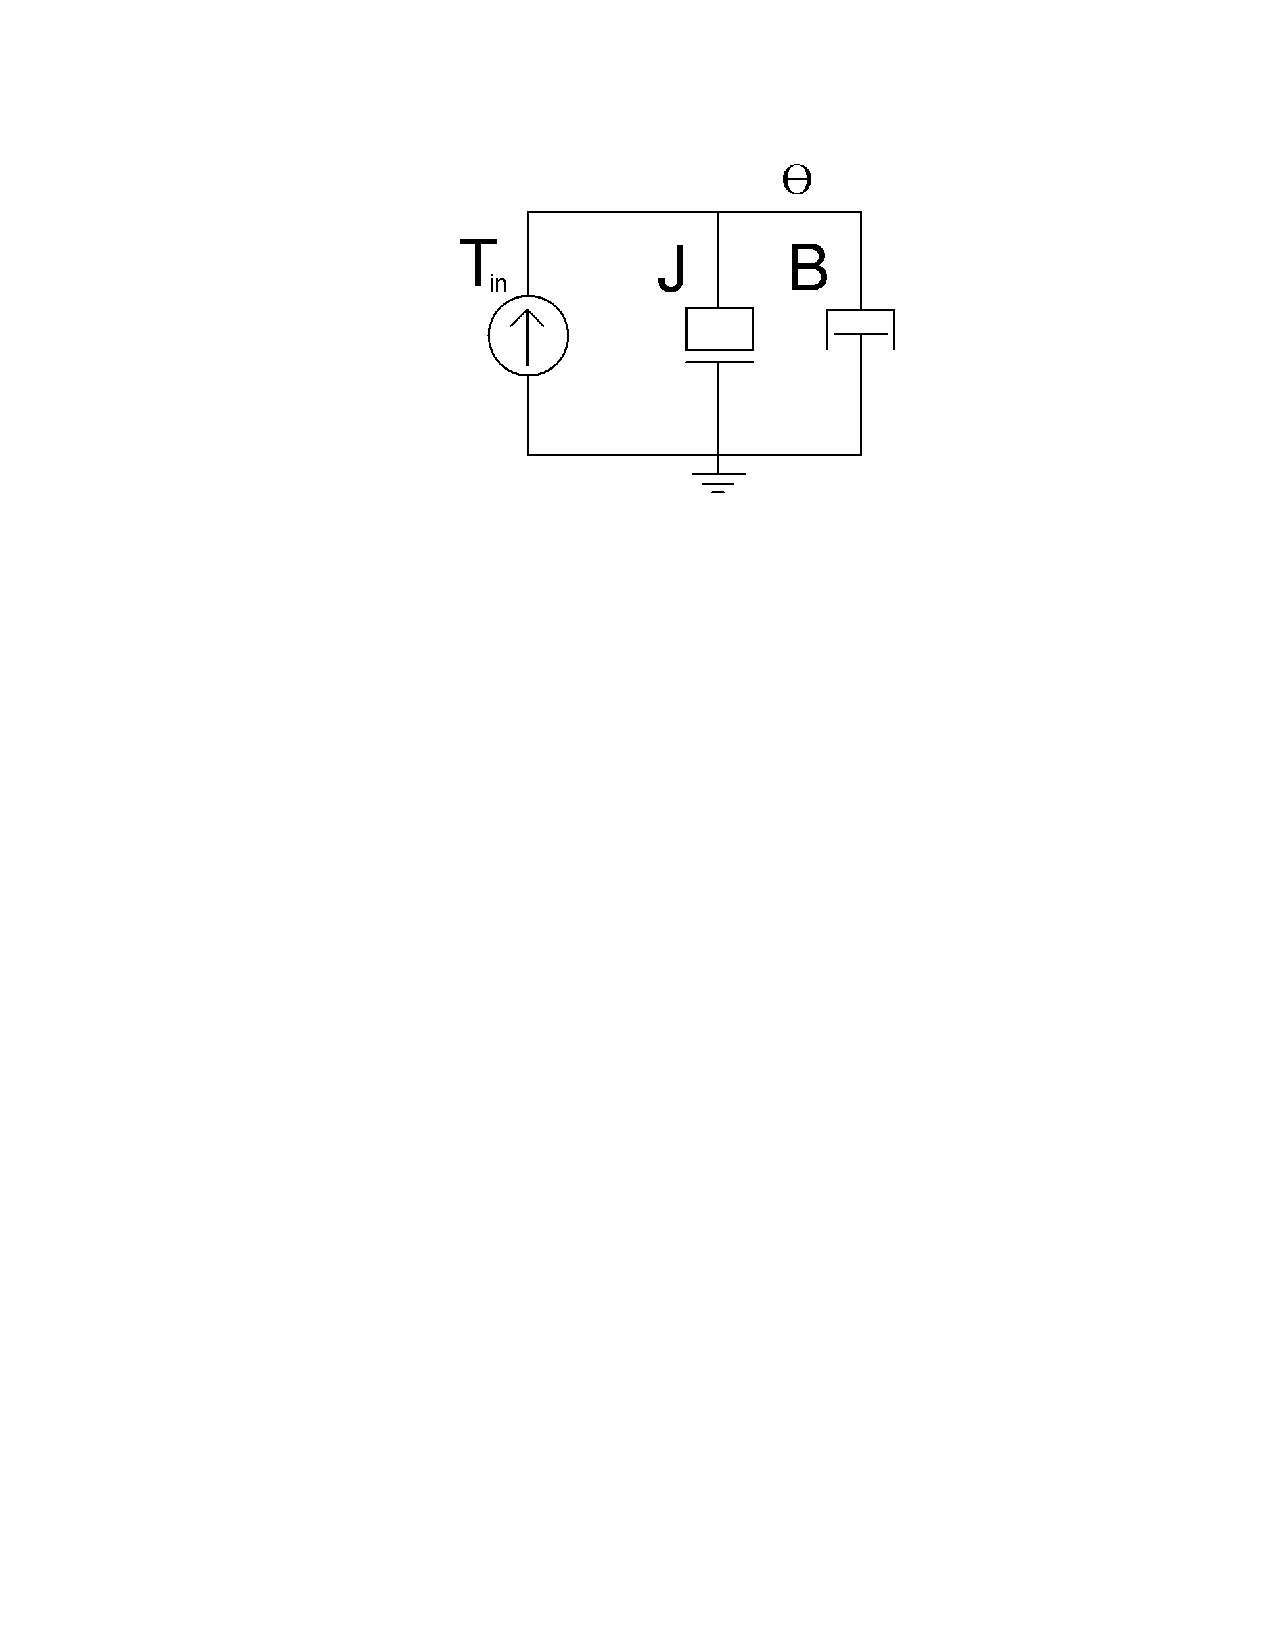
\includegraphics[width=0.7\columnwidth]{./pix/smcMech.pdf}
  \caption{Mechanical Schematic Drawling of Reduced System for SMC based on Fig~\ref{fig:couple}}
  \label{fig:smcMech}
\end{figure}

\noindent The dynamic equations for the system in Fig.~\ref{fig:smcSliding} are written as

\begin{equation}
\begin{array}{ccc}
T(t) = J\ddot{\theta}+B\dot{\theta} & \rightarrow & \ddot{\theta} = \frac{1}{J}T(t) - \frac{B}{J}\dot{\theta}
\end{array}
\end{equation}


\noindent to implement the SMC $u$ that consists of the approximation of continuous control $\hat{u}$ combined with a switching mode $Q\mbox{sign}(r)$ that is designed to keep the system on the sliding surface

\begin{equation}
u = \hat{u}-Q\mbox{sign}(r)
\end{equation}

\noindent where $r$ is the sliding surface

\begin{equation}
r = \dot{\tilde{\theta}} + \lambda \tilde{\theta}
\end{equation}

\noindent and

\begin{equation}
\hat{u} = \hat{b}^{-1}\left[\ddot{\theta_d}-\hat{f}-\lambda \dot{\tilde{\theta}}\right]
\end{equation}

\noindent where $d$ denotes the desired state, $\hat{}$ denotes the estimate, $\tilde{}$ denotes the error between the observed state and the desired state, $\lambda$ is a gain chosen on a per-system basis, and the following parameters are defined as

\begin{equation}
\begin{array}{cc}
b=\frac{1}{J}, & R = \frac{B}{J}
\end{array}
\end{equation}

\noindent and

\begin{equation}
\begin{array}{cc}
f=-R\dot{\theta}, & \hat{f}=-R_{ave}\dot{\theta}
\end{array}
\end{equation}


\noindent where bounds on $J$ and $R$ are set as

\begin{equation}
\begin{array}{ccc}
R_{min}\leq R \leq R_{max}, & R_{min} = \frac{B}{J_a+J_L}, & R_{max} = \frac{B}{J_a}
\end{array}
\end{equation}

\noindent The maximum deviation and average value of $R$ is defined by $R_x$ and $R_{ave}$ respectively

\begin{equation}
\begin{array}{cc}
R_{x} = \left|R_{max}-R_{min}\right|, & R_{ave} = \frac{1}{2}\left(R_{max}+R_{min}\right)
\end{array}
\end{equation}

values of $Q$ mus be sufficiently large so that it stays on the sliding surface

\begin{equation}
Q\geq \hat{b}^{-1}\left(\eta-F\right)+\left(\beta-1\right)\left|\hat{u}\right|
\end{equation}

\noindent where

\begin{equation}
\begin{array}{ccc}
F\geq \left|f-\hat{f}\right| & \rightarrow & F=R_x\left|\dot{\theta}\right|
\end{array}
\end{equation}

\noindent and


\begin{equation}
\begin{array}{ccc}
\beta=\left(\frac{b_{max}}{b_{min}}\right)^{\frac{1}{2}}, 	& 	b_{min}= \frac{1}{J_a+J_L}, 	& b_{max} = \frac{1}{J_a}
\end{array}
\end{equation}

\noindent and $\hat{b}$ (the estimate of $b$) is the geometric mean of $b$. 
The values $\eta$ and $\lambda$ are restricted by the sampling rate of the controller. 
Both of the latter values are not to
exceed a numerical value of half the sampling frequency in Hz.
Fig.~\ref{fig:danBode} shows the frequency response of SMC on the TR system

Multiple simulations were made on the SMC control method to reduce the effects of TR. Table~\ref{table:resultsClosedLoop} shows the
results of these test for multiple ratios of $J_L:J_a$.  
It is apparent from the simulations that the system will track the desired waveform. 
Load switching has no effect on the system as long as the apparent load stays between $J_{min}$ and $J_{max}$.
As the ration $\frac{J_L}{J_a} \rightarrow 0$ the effect of TR on both the magnitude and the phase goes to zero.
To motor position $\theta_a$ and motor velocity $\dot{\theta}_a$ are needed to preform proper SMC in a TR system. 

%\section{Results}\label{sec:results}


\begin{center}
	\begin{table}
	\caption{Effects of changing the ratio of $J_L:J_a$ (Open Loop) $K_c=55.0\frac{oz}{in}$}
	\begin{center}
  \begin{tabular}{  c | c | c | c }

Ratio					& $J_L$										& $\Delta dB$	& $\Delta$ TR Phase \\ 
($J_L:J_a$)		&($oz\cdot in\cdot sec^2$)& ($dB$)			& ($deg$)							\\	\hline
\hline
2.000  				&0.00460  								&9.542  			&180.0							\\	\hline
1.435  				&0.00330  								&7.729  			&180.0							\\	\hline
0.500  				&0.00115  								&3.522  			&180.0							\\

  \end{tabular}
  \end{center}
  \label{table:resultsOpenLoop}
  \end{table}
\end{center}


\begin{center}
	\begin{table}
	\caption{Effects of changing the ratio of $J_L:J_a$ when using RE and SMC (Closed Loop) $K_c=55.0\frac{oz}{in}$}
	\begin{center}
  \begin{tabular}{ c | c | c | c | c | c }
						&								& 												& 								& $\Delta$ TR 		& $\Delta$ TR 			\\ 
Control			&Ratio					& $J_L$										& $\Delta dB$			& Mag 						& Phase 						\\ 
Method			&($J_L:J_a$)		&($oz\cdot in\cdot sec^2$)& ($dB$)					& ($dB$)					& ($deg$)						\\	\hline
\hline
RE 					&2.000  				&0.00460  								&0.500  					&0.400  					&4.600							\\	\hline
RE 					&1.435  				&0.00330  								&0.300  					&0.200  					&3.500							\\	\hline
RE 					&0.500  				&0.00115  								&0.500  					&0.100  					&1.600							\\	\hline
\hline
SMC 				&2.000  				&0.00460  								&0.000  					&24.652  					&130.840						\\	\hline
SMC 				&1.435  				&0.00330  								&0.000  					&10.200  					&23.770							\\	\hline
SMC 				&0.500  				&0.00115  								&0.000  					&0.012  					&1.815							\\	


  \end{tabular}
  \end{center}
  \label{table:resultsClosedLoop}
  \end{table}
\end{center} 

\begin{figure}[ht]
  \centering
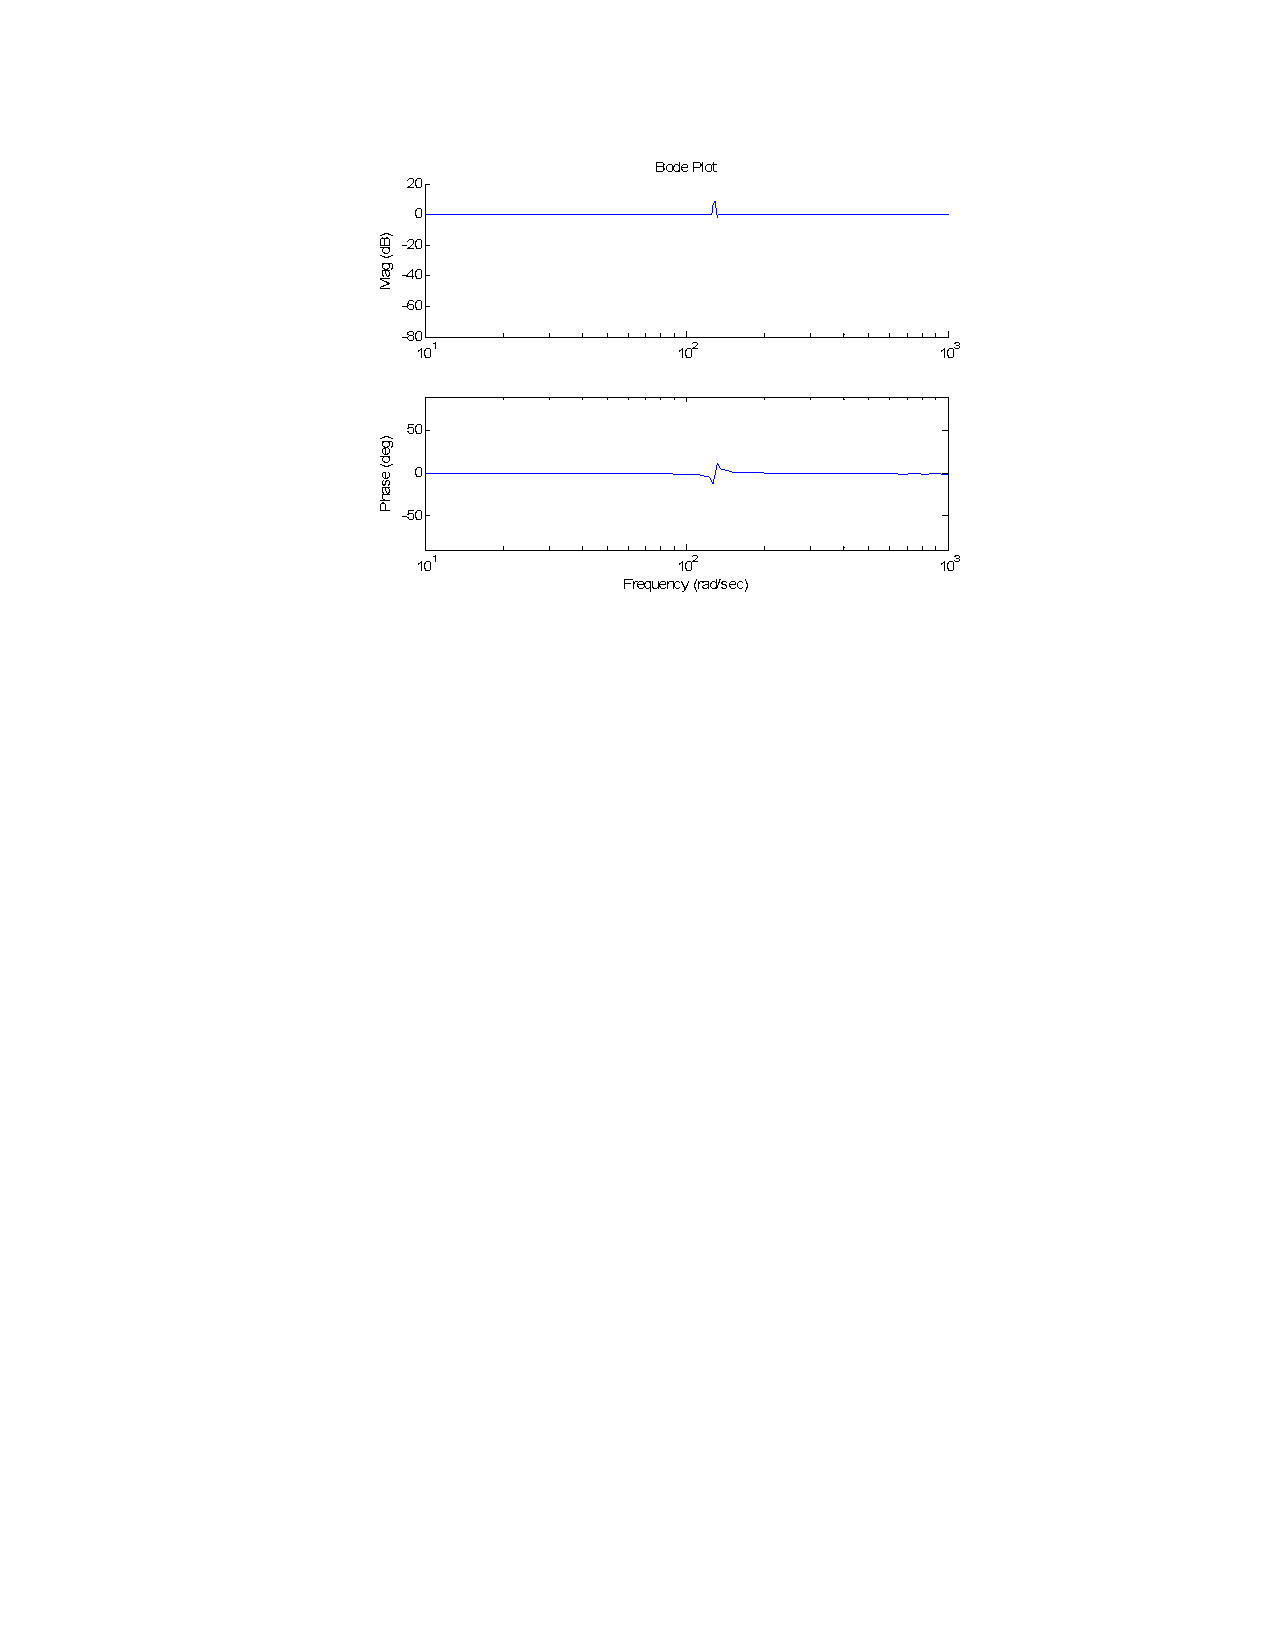
\includegraphics[width=0.8\columnwidth]{./pix/danBode.pdf}
  \caption{Frequency response plot for SMC on system with TR with $\eta= 0.3$ and $\lambda=30,000$}
  \label{fig:danBode}
\end{figure}

%\input{comparison.tex}
%%\section{Results}\label{sec:results}


\begin{center}
	\begin{table}
	\caption{Effects of changing the ratio of $J_L:J_a$ (Open Loop) $K_c=55.0\frac{oz}{in}$}
	\begin{center}
  \begin{tabular}{  c | c | c | c }

Ratio					& $J_L$										& $\Delta dB$	& $\Delta$ TR Phase \\ 
($J_L:J_a$)		&($oz\cdot in\cdot sec^2$)& ($dB$)			& ($deg$)							\\	\hline
\hline
2.000  				&0.00460  								&9.542  			&180.0							\\	\hline
1.435  				&0.00330  								&7.729  			&180.0							\\	\hline
0.500  				&0.00115  								&3.522  			&180.0							\\

  \end{tabular}
  \end{center}
  \label{table:resultsOpenLoop}
  \end{table}
\end{center}


\begin{center}
	\begin{table}
	\caption{Effects of changing the ratio of $J_L:J_a$ when using RE and SMC (Closed Loop) $K_c=55.0\frac{oz}{in}$}
	\begin{center}
  \begin{tabular}{ c | c | c | c | c | c }
						&								& 												& 								& $\Delta$ TR 		& $\Delta$ TR 			\\ 
Control			&Ratio					& $J_L$										& $\Delta dB$			& Mag 						& Phase 						\\ 
Method			&($J_L:J_a$)		&($oz\cdot in\cdot sec^2$)& ($dB$)					& ($dB$)					& ($deg$)						\\	\hline
\hline
RE 					&2.000  				&0.00460  								&0.500  					&0.400  					&4.600							\\	\hline
RE 					&1.435  				&0.00330  								&0.300  					&0.200  					&3.500							\\	\hline
RE 					&0.500  				&0.00115  								&0.500  					&0.100  					&1.600							\\	\hline
\hline
SMC 				&2.000  				&0.00460  								&0.000  					&24.652  					&130.840						\\	\hline
SMC 				&1.435  				&0.00330  								&0.000  					&10.200  					&23.770							\\	\hline
SMC 				&0.500  				&0.00115  								&0.000  					&0.012  					&1.815							\\	


  \end{tabular}
  \end{center}
  \label{table:resultsClosedLoop}
  \end{table}
\end{center}

 \section{Conclusion}
The two different control designs for reducing the effect of TR in coupled systems, RE and SMC, both
reduce the effect greatly. Table~\ref{table:resultsClosedLoop} shows the results from the control using RE 
and the control using SMC. These results show that RE reduces the TR Mag Change over a
greater range than SMC does. However SMC has a $\Delta dB$ of $0dB$ over all of the ratios of $J_L:J_a$ while RE
continues to have the switching effect.
 
 
 

\FloatBarrier
\bibliographystyle{IEEEtran}
%\bibliographystyle{plain}
\bibliography{tr}{}
  
%\end{thebibliography}




% that's all folks
\end{document}


